We begin our empirical analysis of the model by first applying the subgraph localization procedure by itself (standalone), separate from our manifold regression scheme. In this case, our statistic is derived from {\em only} Generalized Linear Models (GLM) constructions, where the $\hat{\Bbeta}_g^R$ in equation \eqref{eq:LRstat} is the slope estimated from fitting standard first order linear models. Identifying the differentially varying subgraphs across groups in this way is similar to a simpler version of the planted clique identification problem \citep{arora2009computational}, where the clique we are trying to identify corresponds to those nodes whose slopes vary significantly across groups.
\begin{figure}
	\begin{center}
		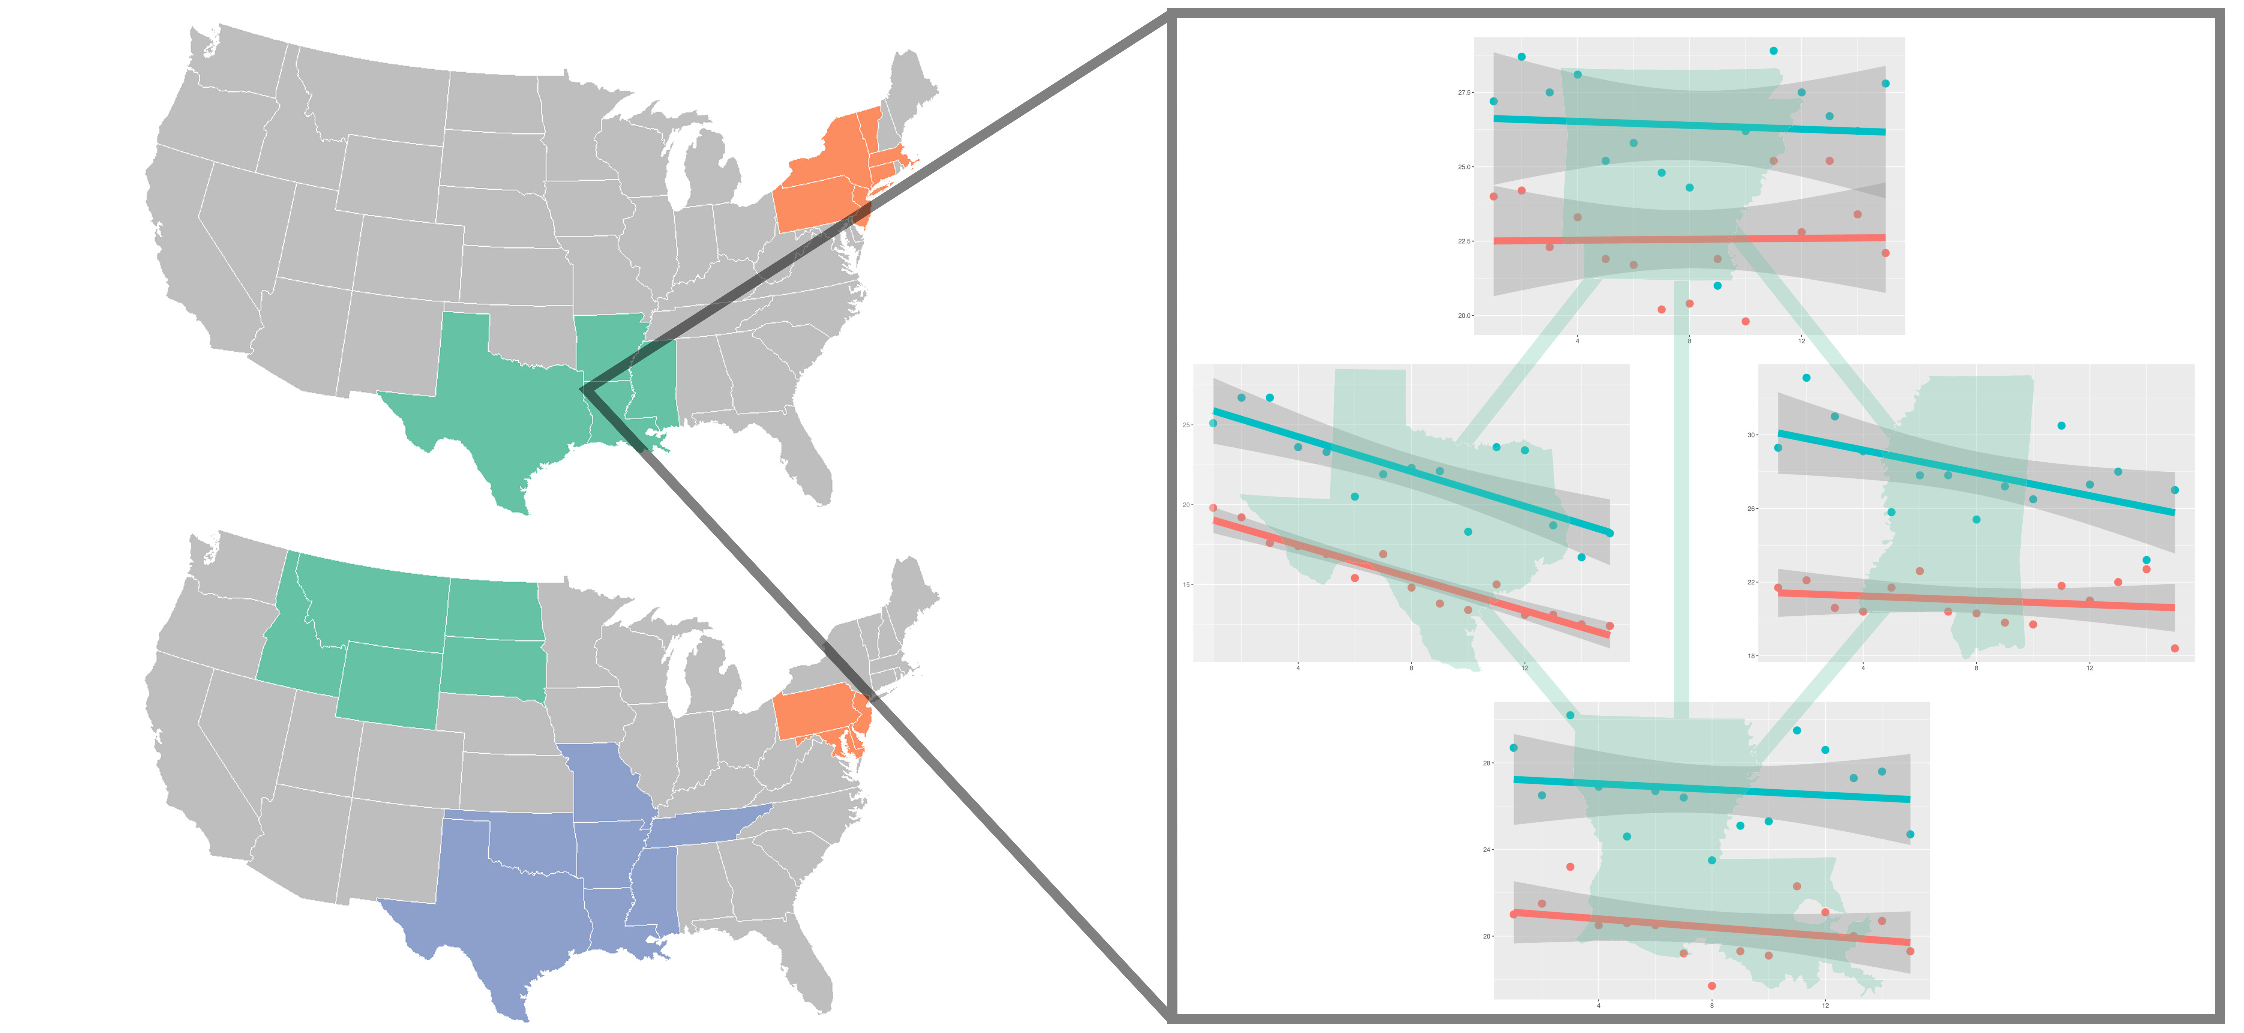
\includegraphics[trim={0cm 0cm 0cm 0cm}, clip, width=0.9\textwidth]{3_covtraj/figs/tobacco_zoom.pdf}
	\end{center}
	\caption[Tobacco use state relationships via covariance trajectory analysis]{(left,top) States identified as having significantly different time-varying tobacco usage across gender from 2001 to 2015. (left,bottom) States identified as having significantly different time-varying heavy drinking use across gender from 2010 to 2015. (right) Linear regressions over tobacco usage fitted to the four states defined by the ball subgraph centered at Louisiana. Best viewed in color.}
	\label{fig:tobalc}
\end{figure}

{\em Data.} The Center for Disease Control (CDC) provides extensive statistics regarding tobacco and alcohol usage across the US. This data has been collected systematically for the last few decades and is publically available (includes demographic information and gender). As a simple application of our 
proposed framework, 
we may pose the following question: which ``sub-groups'' of states tend to evolve differently in their correlation (pertaining to tobacco/alcohol usage) over time? 
Our framework extends easily to answer this question. In this setup, the oracle graph is simply the adjacency graph of the continental
US naturally which will be used directly in our scanning procedure.
For this dataset, we have direct observations of node measures: the percentage of males and females who 
reported smoking or drinking heavily in each state. Using 
gender as the group, 
we fit standard linear models for each candidate subgraph, and compute the difference of gender-wise 
slopes statistic as described above. 
In Figure \ref{fig:tobalc}, we see the regions identified using our method, and interpret some of the tobacco usage findings here.

In the northeast, we see that women have reduced their tobacco usage at a significantly faster rate than men compared to the rest of the country. 
%http://www.who.int/bulletin/archives/78(7)891.pdf
We suspect that this may be at least partly tied to the development of women's cigarette brands in the late 1960s and 1970s 
followed by subsequent aggressive public policy campaigns in the 1990s and 2000s to highlight health risks beyond 
pulmonary or cardiovascular diseases for women (e.g., infertility, reduced bone-density in post-menopausal women). We also see that 
state-wide indoor smoking bans were put in place in the Northeast 
%\href{https://en.wikipedia.org/wiki/List_of_smoking_bans_in_the_United_States}{(2003/2004)} 
ahead of many other states in the union.  
In the South, the trends among men and women also seems to differ significantly. (see Figure \ref{fig:tobalc}). 
Apart from health factors, the group-wise differences in the group-wise trends may also be explained by 
a few reasons identified in a study in 2007 \citep{HEC:HEC1223} which found that as the state sales tax on cigarettes changed (increased), 
women were significantly more price elastic than men. Between 2006 and 2008, the cigarette tax increased dramatically for all of the 4 states identified \textit{except for Louisiana}, whose tax rate has remained constant. Additionally, while Arkansas did increase their cigarette tax in 2009, they did \textit{not increase taxes in locations near borders shared with higher taxing states}. These intricate relationships among states lend credibility to the fact that our scan statistics framework is indeed identifying interesting sub-regions, and suggests that the full covariance-trajectory pipeline may be more appropriate if effects beyond the means are relevant within an analysis. 

%With heavy alcohol usage in the South, West, and Northeast, the prevalence of heavy drinking seems to be declining faster in men. 
%
